
\documentclass[a4paper,12pt]{article}
\usepackage{times}
\usepackage[francais]{babel}
\usepackage[utf8x]{inputenc}
\usepackage[T1]{fontenc}
\usepackage{amsmath}
\usepackage{amssymb}
\usepackage{graphicx}
\usepackage{pdfpages}
\usepackage{pdflscape}
\usepackage{listings}
\usepackage{longtable}
\lstset{literate=
{é}{{\'e}}1
{è}{{\`e}}1
{ê}{{\^e}}1
{à}{{\`a}}1
{â}{{\^a}}1
}
\lstset{language=C++,
basicstyle=\footnotesize,
keywordstyle=\footnotesize\color{blue},
otherkeywords={override,nullptr}
}
\definecolor{orange}{rgb}{0.8,0.4,0.0}
\definecolor{darkblue}{rgb}{0.0,0.0,0.6}
\definecolor{cyan}{rgb}{0.0,0.6,0.6}
\lstdefinelanguage{JSON}
{
basicstyle=\normalsize,
columns=fullflexible,
showstringspaces=false,
commentstyle=\color{gray}\upshape,
morestring=[b]",
morestring=[s]{>}{<},
morecomment=[s]{<?}{?>},
stringstyle=\color{orange},
identifierstyle=\color{darkblue},
keywordstyle=\color{blue},
morekeywords={string,number,array,object}% list your attributes here
}

\sloppy

\setlength{\topmargin}{0cm}
\setlength{\headsep}{0.in}
\setlength{\headheight}{0.in}
\setlength{\evensidemargin}{0cm}
\setlength{\oddsidemargin}{-1cm}
\textwidth 18cm
\textheight 25cm

\begin{document}

    \thispagestyle{empty}

    \begin{titlepage}

        \vspace*{2cm}

        \begin{center}\textbf{\Huge Projet Logiciel Transversal}\end{center}{\Large \par}

        \begin{center}\textbf{\large Anand Candassamy \& Paul Estano}\end{center}{\large \par}

        \vspace{2cm}

        \clearpage

        {\small
        \tableofcontents
        }

    \end{titlepage}

    \clearpage
    \section{Présentation Générale}

    \subsection{Archétype}
	    Notre jeu s'inspirera principalement du jeu \emph{Pokemon Donjon Mystère}. En effet, nous avons prévu de conserver le mécanisme des combats et de donjon de ce jeu.
	    \\Dans notre logiciel l'utilisateur incarnera un pokemon dans les salles d'un donjon qui contiennent chacune des pokemons qui peuvent l'"agresser". Le nombre de pokemons dans une salle évolue en fonction de l'avancement du joueur dans le jeu. 
	    \\Pour simplifier le jeu nous abandonnons également d'évolution des pokemons.

    \subsection{Règles du jeu}
	  Le donjon contient un nombre fini de salles et le joueur gagne lorsqu'il sort de la dernière salle du donjon.
	  Un donjon a 10 salles, le pattern de chaque étage n'est pas tiré aléatoirement. Le joueur a la possibilité d'accéder à des étages bonus, dîtes arène de combat où il pourra se battre contre un autre joueur en ligne.
	   \\Le joueur est provoqué en duel automatiquement par les pokemons qui sont autour de lui. Il faut qu'il tue l'IA ou le joueur adverse pour activer la case de l'esaclier qui leur permet de passer à l'étage suivant.
\\Les combats fonctionnent en tour par tour. A chaque tour, l'utilisateur peut effectuer une action :
\begin{itemize}
    \item attaquer avec une compétence
    \item soigner le pokemon
    \item se déplacer d'une case
\end{itemize}
\clearpage
    \subsection{Ressources}
    \begin{figure}[ht]
    \begin{center}
        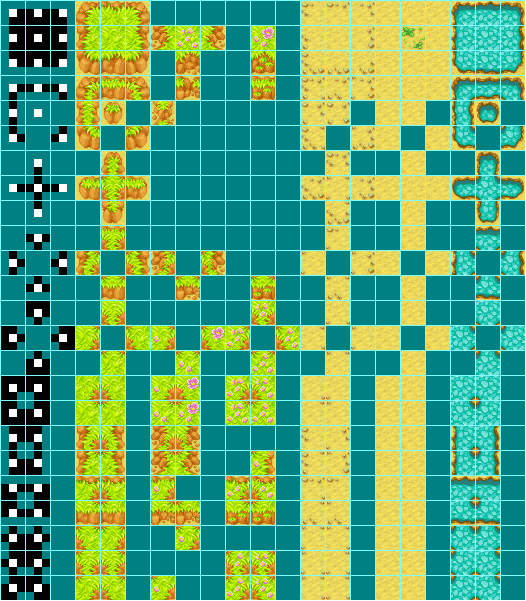
\includegraphics[width=0.8\textwidth]{tilemap.png}
    \end{center}
    \caption{Tileset utilisé pour construire un monde}
    \end{figure}
    
    \begin{figure}[ht]
    \begin{center}
        
\includegraphics[width=0.8\textwidth]{pokemonLatex.png}
    \end{center}
    \caption{Tileset utilisé pour les pokémons}
    \end{figure}



    \clearpage
    \section{Description et conception des états}
    
    \subsection{Description des états}
    Un état du jeu est formé d'une carte qui est statique au cours du temps et d'une liste de joueurs dont l'état varie au cours du jeu.
    
     \subsubsection{État de la carte}
     
     La carte est un élément fixe de l'état du jeu. Il se décompose en plusieurs cases.
    
     Les cases se distinguent en 3 parties : \begin{itemize}
    \item les murs, qui ne sont pas franchissables par les éléments mobiles.
    \item les cases "conteneurs", elles peuvent être vide ou occupé par un seul élément mobile.
    \item les cases escaliers, il en existe un seul par étage, qui permet d'aller au niveau suivant du labyrinthe.
    
    \end{itemize}

    \subsubsection{État des joueurs}
    Un pokemon est soit contrôlé par un joueur soit contrôlé par une Intelligence Artificielle (I.A), il possède une position, un nombre de points de vie à l'état t, un nom et un ensemble de statistiques qui lui sont attribués en début de partie. Le pokemon est considéré comme étant "mort" si son nombre de points de vie atteint 0.
    
    \subsubsection{État général}
    A l’ensemble des éléments statiques et mobiles, nous rajoutons les propriétés suivantes :
    — Époque : représente « l’heure » correspondant à l’état, ie c’est le nombre de « tour » passés
    globale depuis le depuis de la partie.

    
    Ces statistiques correspondent aux attaques qu'il peut utiliser, à son nombre de point de vie en début de partie et son type (Salameche, Bulbizarre, Carapuce).
    \subsection{Conception Logiciel}
    Le package état peut se diviser en trois sous-partie:\begin{itemize}
        \item Une partie gérant les personnages, en bleu
        \item Une partie gérant l'environnement, en rouge
        \item Une classe représentant l'état global du jeu, en vert
    \end{itemize}
    
     La classe \emph{Player} contient l'ensemble des éléments permettant de caractériser l'état d'un joueur. Chaque joueur est lié à un pokemon par une relation de composition : un pokemon ne peut pas exister sans joueur. Dans le cas où le pokemon est contrôlé par l'IA, l'IA est considérée comme un joueur et contrôle donc son pokemon.
    
    Chaque pokemon possède une relation d'agrégation avec des statistiques qui lui sont attribués en début de partie.
    
    Pour notre implémentation du jeu, nous avons prévu d'utiliser que les trois pokémon suivant : \begin{itemize}
        \item Carapuce
        \item Salamèche
        \item Bulbizarre
    \end{itemize}
    Le constructeur respectif de chacun de ces trois pokemons héritent de la classe Pokemon. Nous avons mis en place un identifiant pour chaque pokemon, ce qui permet d'avoir plusieurs pokemon construit à partir de la même classe.
    
    La partie environnement est calqué sur le modèle proposé par les fichiers exportés par le logiciel \emph{Tiled Map Editor} au format JSON. Les objets les plus consommateurs en mémoire tels les \emph{data} dans la classe \emph{Layer} sont par ailleurs stockés dans le tas pour éviter les copies entre les différentes classes.
    
     L'état global contient un pointeur vers l'état de l'environnement et et une liste de pointeur de contenant l'état des différents joueurs de la partie. Un booléen permettant de détecter la fin du jeu a également été ajouté. 
     
     On utilise le pattern \emph{Observer} pour notifier les éléments dépendant de l'état lorsque celui-ci change. La classe \emph{State} hérite de la classe \emph{Observable} qui contient une liste d'objets héritant de la classe abstraite \emph{Observer}. Lorsque la classe \emph{State} subit un changement, l'utilisateur utilise la méthode \emph{notifyObservers()} pour notifier ses observers avec l'évènement correspondant au changement appliqué.
     Il existe 2 types d'\emph{Event}:
\begin{itemize}
\item Les \emph{TAB\_EVENT} qui représente un changement d'état lié aux joeurs (mort, changement de position , changement d'orientation)
\item Les \emph{STATE\_EVENT} qui correspondent à des changement liés à l'environnement (changement de niveau) ou à des changements liéés aux statistiques de la partie
\end{itemize}
     d{itemie}
  Afin d'éviter des problèmes techniques suite à notre implémentation, nous avons mis en place des fonctions afin de capturer les exceptions rencontrées lors de l'exécution, principalement dans la classe qui charge les données de la carte. De plus nous avons utilisés des entiers signé afin que les valeurs et statistiques des pokemons ne prennent jamais de valeurs négatives.
     
     Nous avons pour l'instant implémenter que les fonction set et get qui permettent d'instancier nos objets liés aux états . 
    \begin{landscape}
    \begin{figure}[p]
    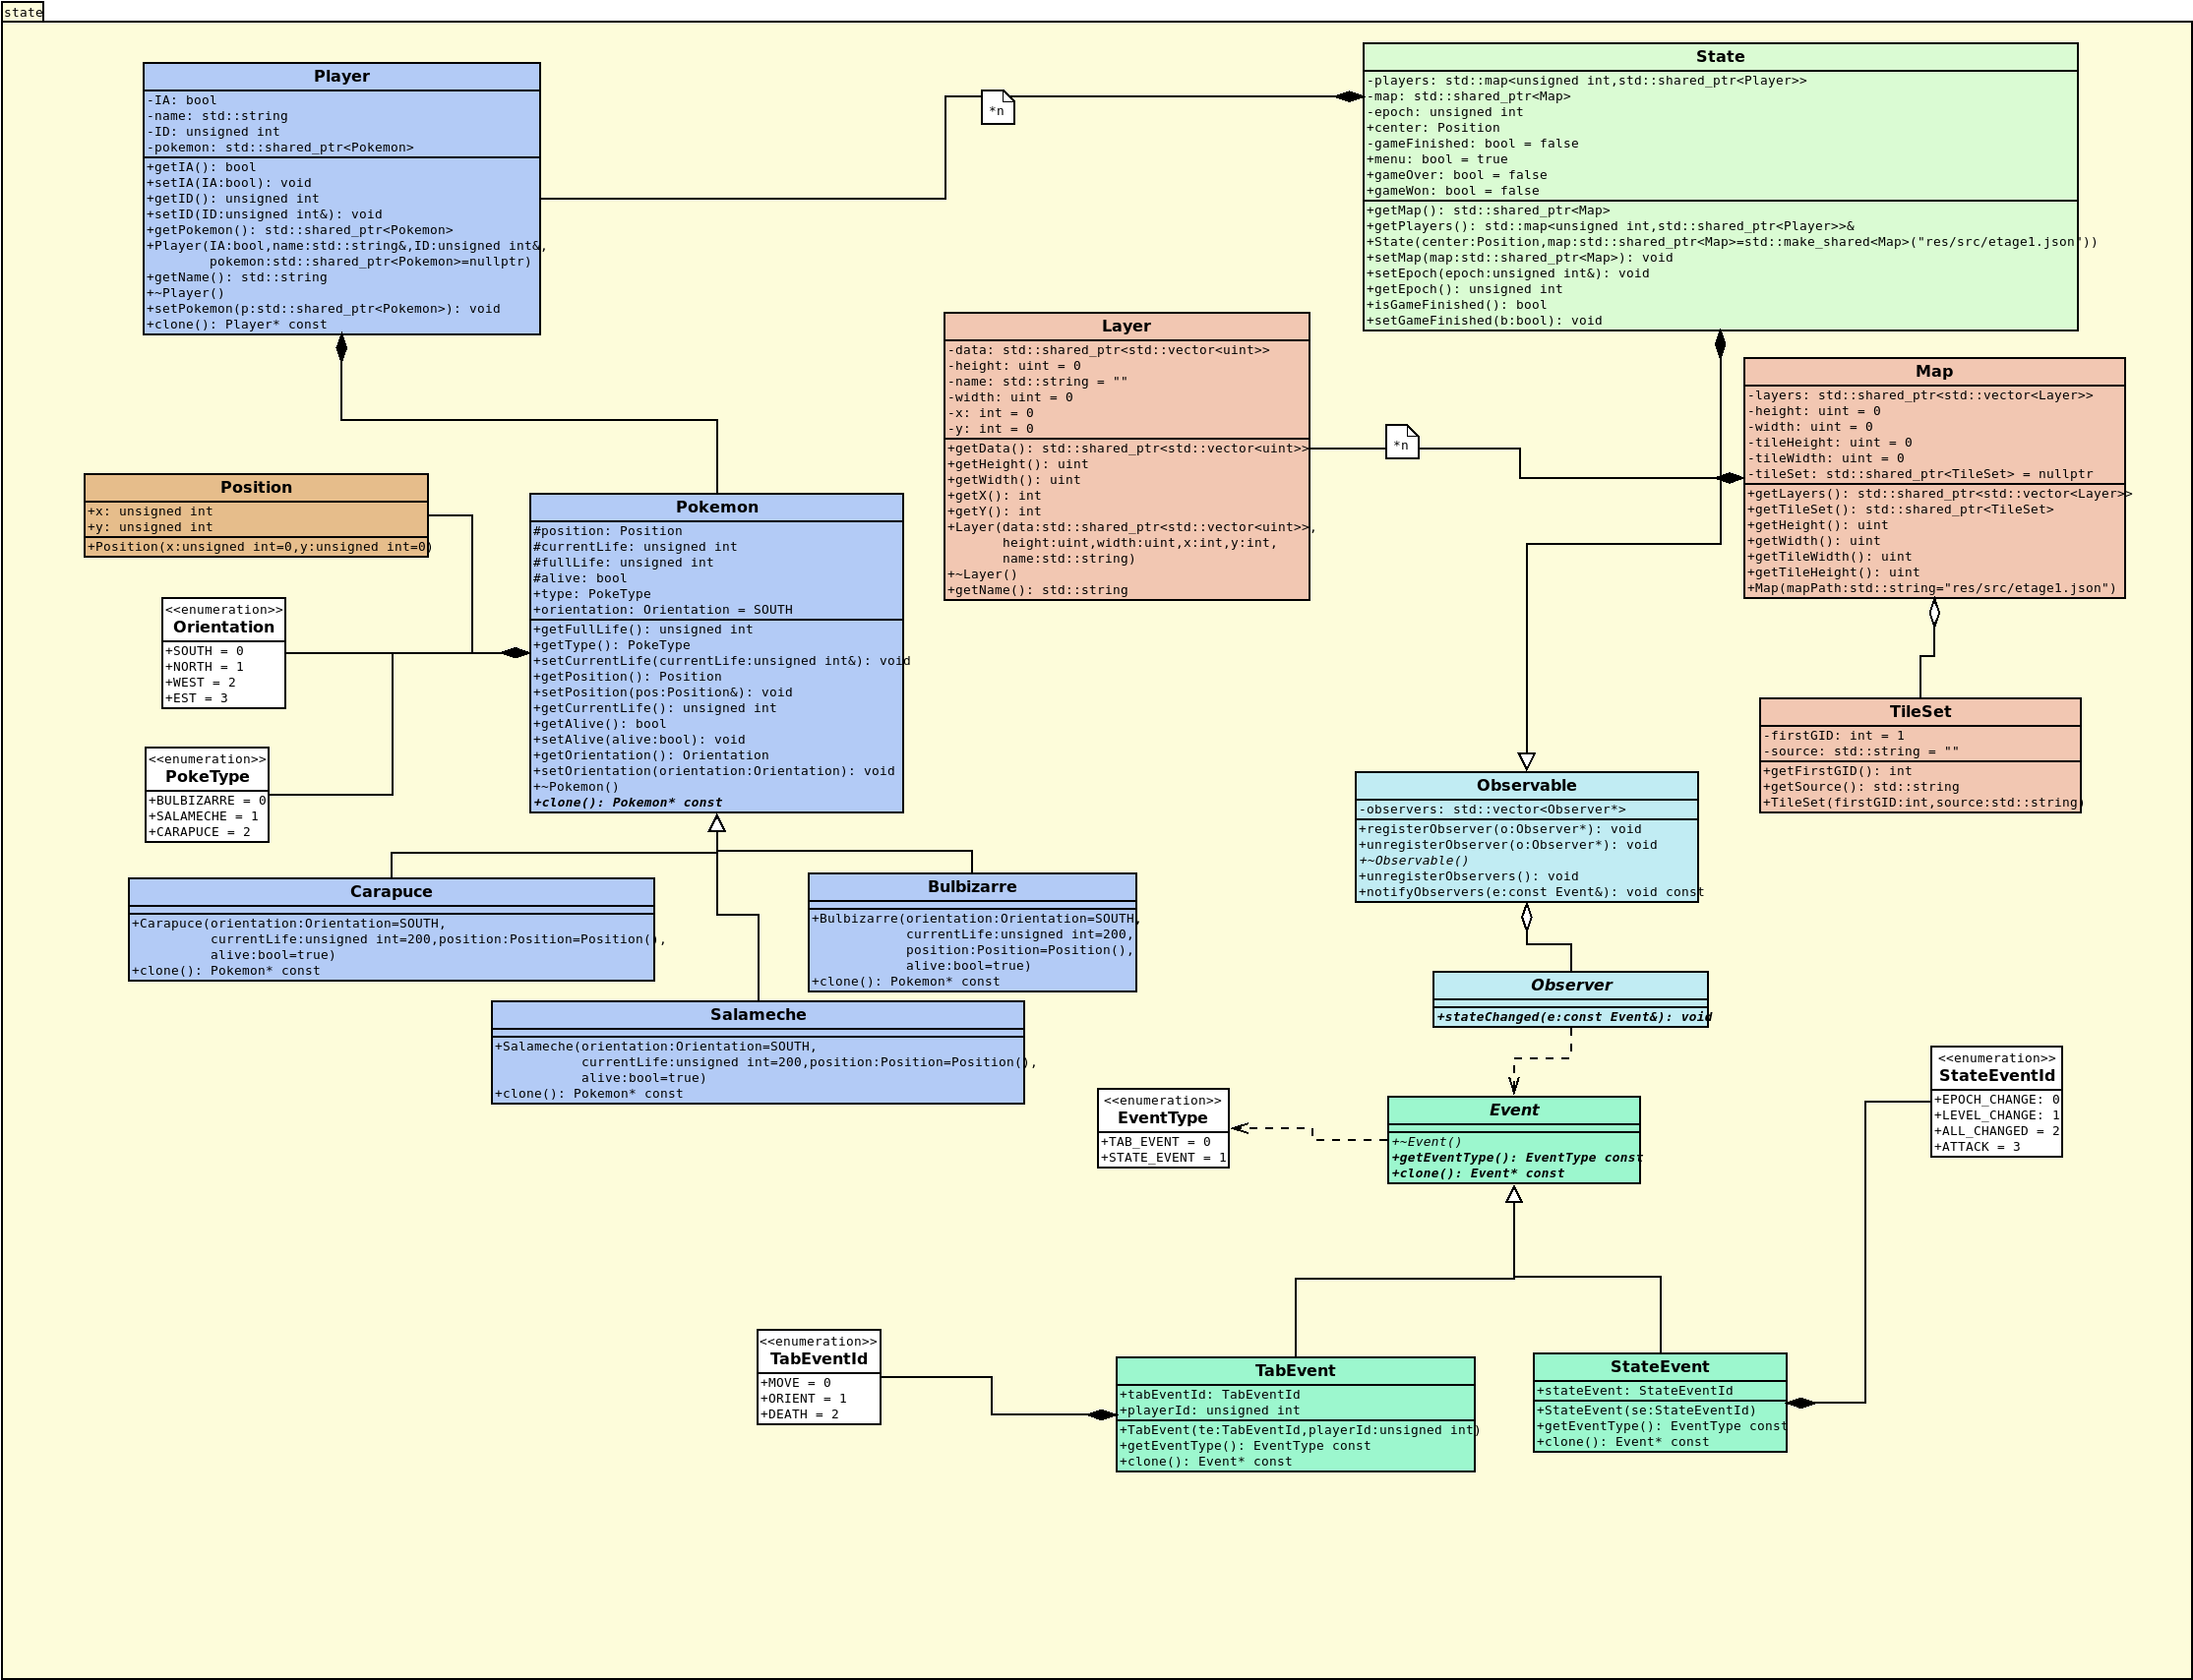
\includegraphics[width=0.8\paperheight]{state.png}
    \caption{\label{uml:state}Diagramme des classes d'état.}
    \end{figure}
    \end{landscape}
    \clearpage
    
    
    \section{Rendu: Stratégie et Conception}

    \subsection{Stratégie de rendu d'un état}
    
Notre stratégie de rendu d'un état se base sur l'utilisation de l'interface SFML qui s'appuie sur OpenGL afin de générer un rendu en 2D. Nous avons utiliser les fonctions de SFML afin de charger dans le processeur, la liste des éléments à afficher par le processeur graphique. 
    
Nous avons découper notre affichage graphique sur deux niveaux, la carte avec les éléments décoratifs (mur, sol, escalier) et les éléments mobiles à savoir les pokemons (Carapuce, Salamèche, Bulbizarre) qui se superpose sur le claque précédent. On transmet l'état du jeu ainsi que les textures de toute la carte avec leurs coordonnées et la texture des pokemons avec leurs coordonnées et leur orientation à afficher.
        
La carte étant très grande, nous avons entièrement chargé dans la mémoire pour l'affichage et on a crée une vue (un zoom) centrée sur le pokemon du joueur qui évolue sur la carte, car le but du jeu reste avant tout d'évoluer dans un labyrinthe.
     
Lorsque qu'un changement d'état se produit, la vue est modifiée en fonction du changement appliqué à l'état. Si le changement modifie uniquement la position des pokemon, seule le rendu des pokemon est mis à jour, si ce changement s'applique à l'environnement l'ensemble du rendu de la carte est mis à jour. Lorsque l'ensemble de l'état est modifié le rendu de l'état est entièrement mis à jour. Dans le cas où le jeu est fini la fenêtre est automatiquement fermée.

Nous avons rajouter sur la scène finale, les statistiques des pokemon (point de vie actuelle et id des pokemon) en haut à gauche. 
        
Pour simplifier au mieux notre logiciel, nous n'avons pas inclut les animations de déplacements lorsque le pokemon évolue d'une case à l'autre ainsi que les animations d'attaques quand un pokemon lance une compétence sur un autre.


    \subsection{Conception logiciel}
Pour afficher un état on crée une scène qui génère instancie un ensemble de pointeurs sur des objets graphiques de types \emph{LayerRender} pour la carte.
Pour les Pokemon, on instancie un \emph{Sprite} par Pokemon. Ce \emph{Sprite} contient à la fois les coordonnées du Pokemon sur la fenêtre et sa position sur le Tileset utilisé. Puis, on utilise la méthode \emph{Scene::draw()} pour déclencher l'ouverture de la fenêtre et l'affichage de l'état.
Il est à noter que l'état contient d'ores et déjà toutes les informations nécessaires à l'affichage de la carte. En effet, à la création de l'état celui-ci parse un fichier JSON (ici \emph{map.json})contenant toutes les informations nécessaires à l'affichage de la carte.

 classe \emph{Scene} est un des \emph{Observer} de \emph{State}. Ainsi, lorsque l'état subit un changement, \emph{Scene} est notifié et met à jour le rendu en fonction du type d'évènement qui lui est transmis:
\begin{itemize}
\item Si un \emph{TAB\_EVENT} (correspondant à changement d'état pour l'un des joueurs) la méthode \emph{updatePlayers()} responsable de la mise à jour du rendu des pokemon est appelée.
\item Si un \emph{STATE\_EVENT} (correspondant changement d'état lié à l'environnement ou à la partie) les méthodes \emph{updatePlayers()} et \emph{updateMap()}.
\end{itemize}
Par ailleurs, les points de vie de chacun des pokemon sont, pour le moment, affichés et mis à jour en temps réel à l'intérieur de la méthode \emph{draw()} de la classe \emph{Scene}.

Chaque objet \emph{LayerRender} parcourt l'ensemble des tuiles d'un étage de la carte, détecte la position de la tuile sur la ressource graphique (i.e : l'image du tileset) et calcule sa position sur la fenêtre. Pour optimiser les performances seule l'image du tileset est chargée dans une \emph{Texture}, l'objet \emph{LayerRender} conserve seulement la position de chaque tuile de la carte sur cette texture.
Les pokemons sont chacun rendus à l'intérieur d'un \emph{Sprite}.

    \begin{landscape}
    \begin{figure}[p]
    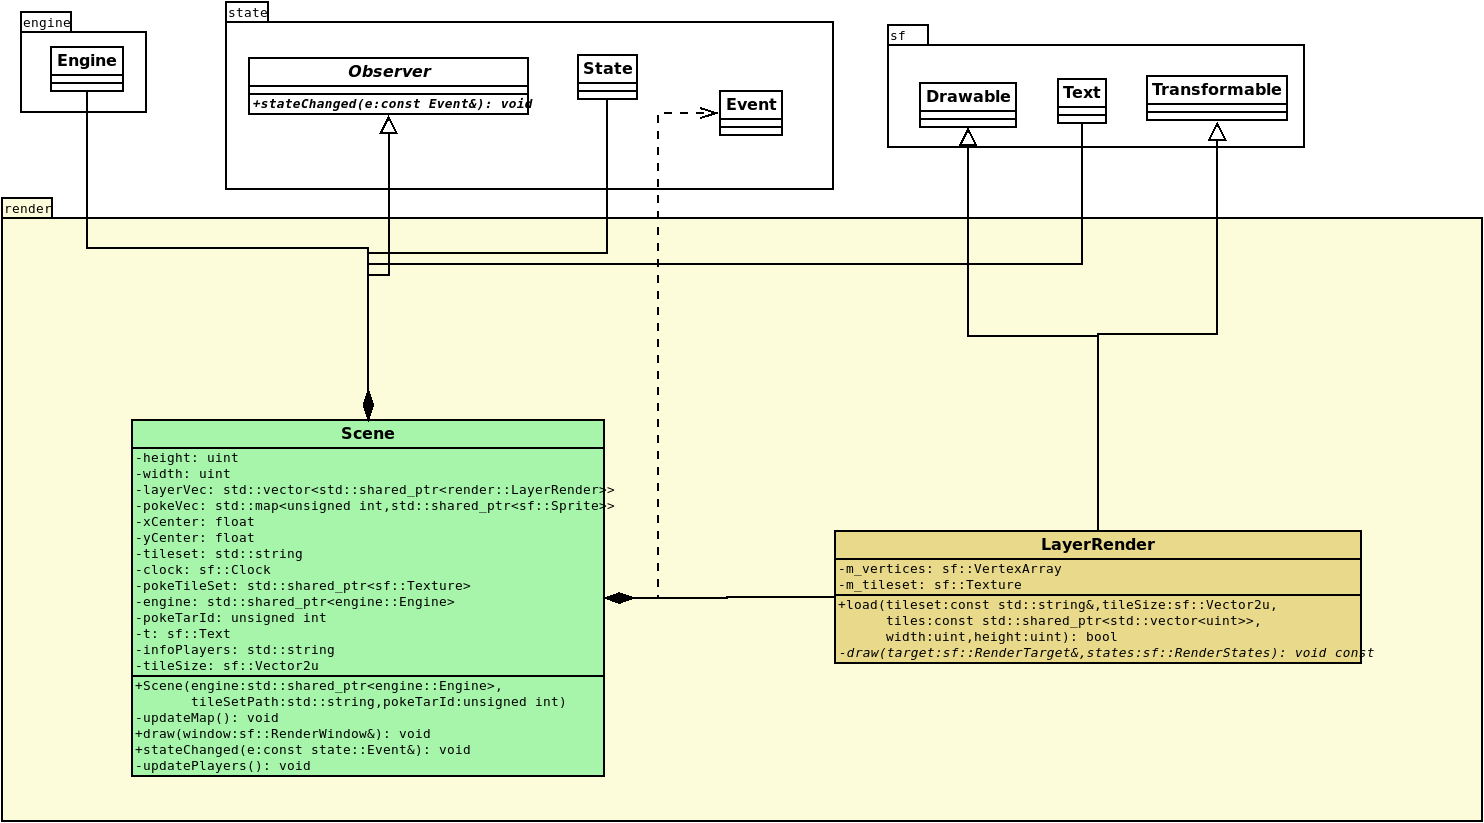
\includegraphics[width=0.9\paperheight]{render.png}
    \caption{\label{uml:render}Diagramme des classes de rendu.}
    \end{figure}
    \end{landscape}

    \clearpage
    \section{Règles de changement d'états et moteur de jeu}

    \subsection{Règles}
    
    Les changements d'états sont liés aux commandes exécutées par le moteur.
    Les commandes extérieures sont : 
    \begin{itemize}
        \item Commande de déplacement
        \item Commande d'attaque
        \item Commande de soin
    \end{itemize}
    
    Une fois qu'une commande extérieure de la part du joueur et de l'IA ont été exécutés (joueur puis IA), on passe au tour suivant.
    
    \subsection{Changements autonomes}
    
    Les changements autonomes interviennent à la fin de chaque changement d'état lié à une commande extérieure et s'exécutent dans l'ordre suivant : 
    \begin{enumerate}
        \item Si le joueur est mort, on affiche "Fin de jeu"
        \item Si l'IA est morte, on active la case escalier pour passer à l'étage suivante
        \item On met à jour les statistiques (point de vie) de l'IA et du joueur en fonction des règles d'attaque et de soin.
        \item On applique les règles de déplacement du joueur et de l'IA. 
        \item Si le joueur est sur la case d'escalier, on vérifie s'il est autoriser à passer au niveau suivant.
    \end{enumerate}
    
    
    
    
    


    \clearpage
    \subsection{Conception logiciel}
On utilise ici le pattern \emph{Command}: un ensemble d'utilisateur peut ajouter des "commandes" à l'objet \emph{Engine} puis lui demander de les exécuter à l'aide de la méthode \emph{runCommands()}.

Les commandes hérite de la classe abstraite \emph{Command} contient une méthode \emph{execute()} virtual pure qui est appelée par le moteur lorsqu'un utilisateur appelle la méthode \emph{runCommands()}. Cette méthode applique en fait directement des changements à l'objet \emph{State} conservé par la classe \emph{Engine}.

On a  implémenté, pour le moment, 3 types de commande:
\begin{itemize}
\item \emph{MoveCommand} qui correspond à un changement de position d'un des pokemon
\item \emph{AttackCommand} qui correspond à l'attaque d'un pokemon
\item \emph{HealCommand} qui est déclenché lorsqu'un joueur veut soigner son pokemon 
\end{itemize}

Les trois commandes \emph{MoveCommand}, \emph{AttackCommand} et \emph{HeakCommand} sont déclencés sur un évènement de lecture de clavier, plus précisement sur un évenement d'appui sur une touche de clavier pour plus de fluidité lors des déplacements dans le parcours du labyrinthe.

La commande \emph{MoveCommand} met à jour le rendu du pokemon sur la map via le render, il redessine la tuile du pokemon suivant son orientation à la bonne case.

Les commandes \emph{AttackCommand} et \emph{HeakCommand} agissent sur l'état des pokemon et sur le rendu de la scène en gardant à jour les points de vie actuels affichés en haut à gauche de la scène.

Par ailleurs, le changement de niveau étant provoqué par un déplacement sur la case escalier après qu'un joueur (non IA) ait éliminé tous ses ennemis; cet évènement est entièrement géré et intégré à la commande \emph{MoveCommand}.

    \begin{landscape}
    \begin{figure}[p]
    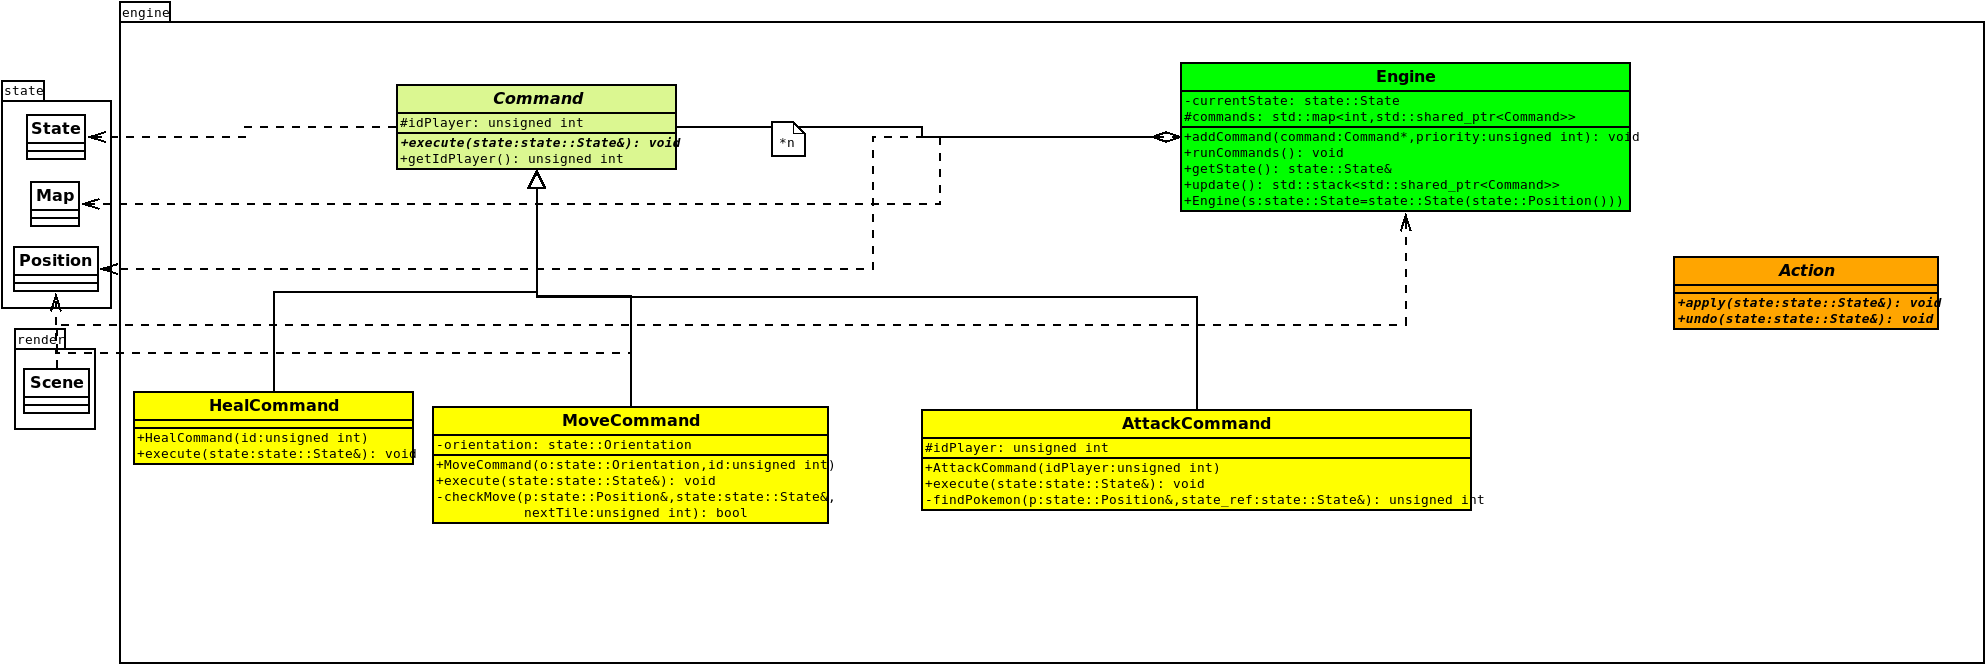
\includegraphics[width=0.9\paperheight]{engine.png}
    \caption{\label{uml:engine}Diagramme des classes de moteur de jeu.}
    \end{figure}
    \end{landscape}


    \section{Intelligence Artificielle}

    \subsection{Stratégies}
    \subsubsection{Intelligence aléatoire}
    
    Le stratégie de l'AI aléatoire est de se déplacer de manière aléatoire sur la map, lors qu'il rencontre un ennemi, il peut alors combattre et lorsque ses pv tombent bas, il se soigne.
    
    \clearpage
    \subsection{Conception logiciel}
    
    Le diagramme des classes d'AI est affiché ci-dessous
    
    \emph{Classes AI}. Les classes filles de la classe AI implémente 3 stratégie d'IA suivi par le pokemon adverse :\begin{enumerate}
        \item RandomAI : Intelligence Artificielle aléatoire
    \end{enumerate}


    \begin{landscape}
    \begin{figure}[p]
    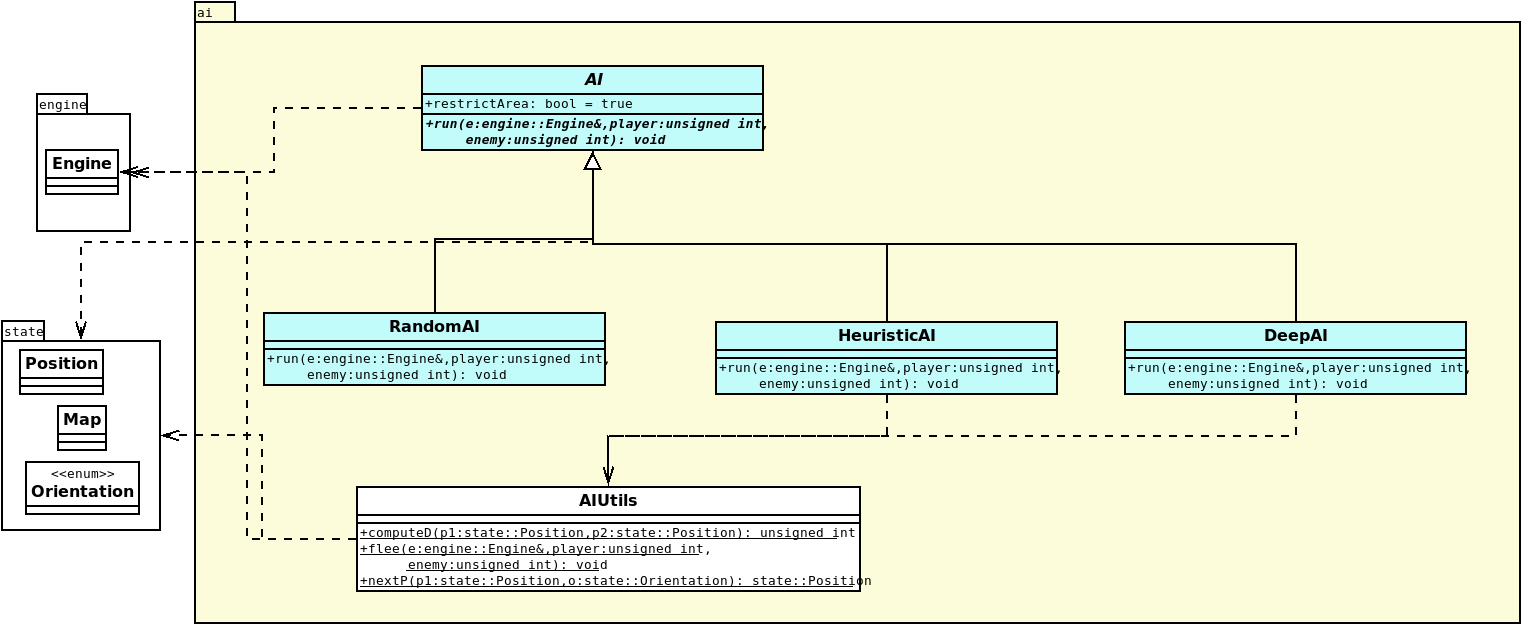
\includegraphics[width=0.9\paperheight]{ai.png}
    \caption{\label{uml:ai}Diagramme des classes d'intelligence artificielle.}
    \end{figure}
    \end{landscape}


    \section{Modularisation}
    \label{sec:module}

    \subsection{Organisation des modules}

    \clearpage
    \subsection{Conception logiciel}
    
    \clearpage
    \section{Annexe}
    \label{sec:Annexe}
    \subsection{Bibliographie}

    %
    %\begin{landscape}
    %\begin{figure}[p]
    %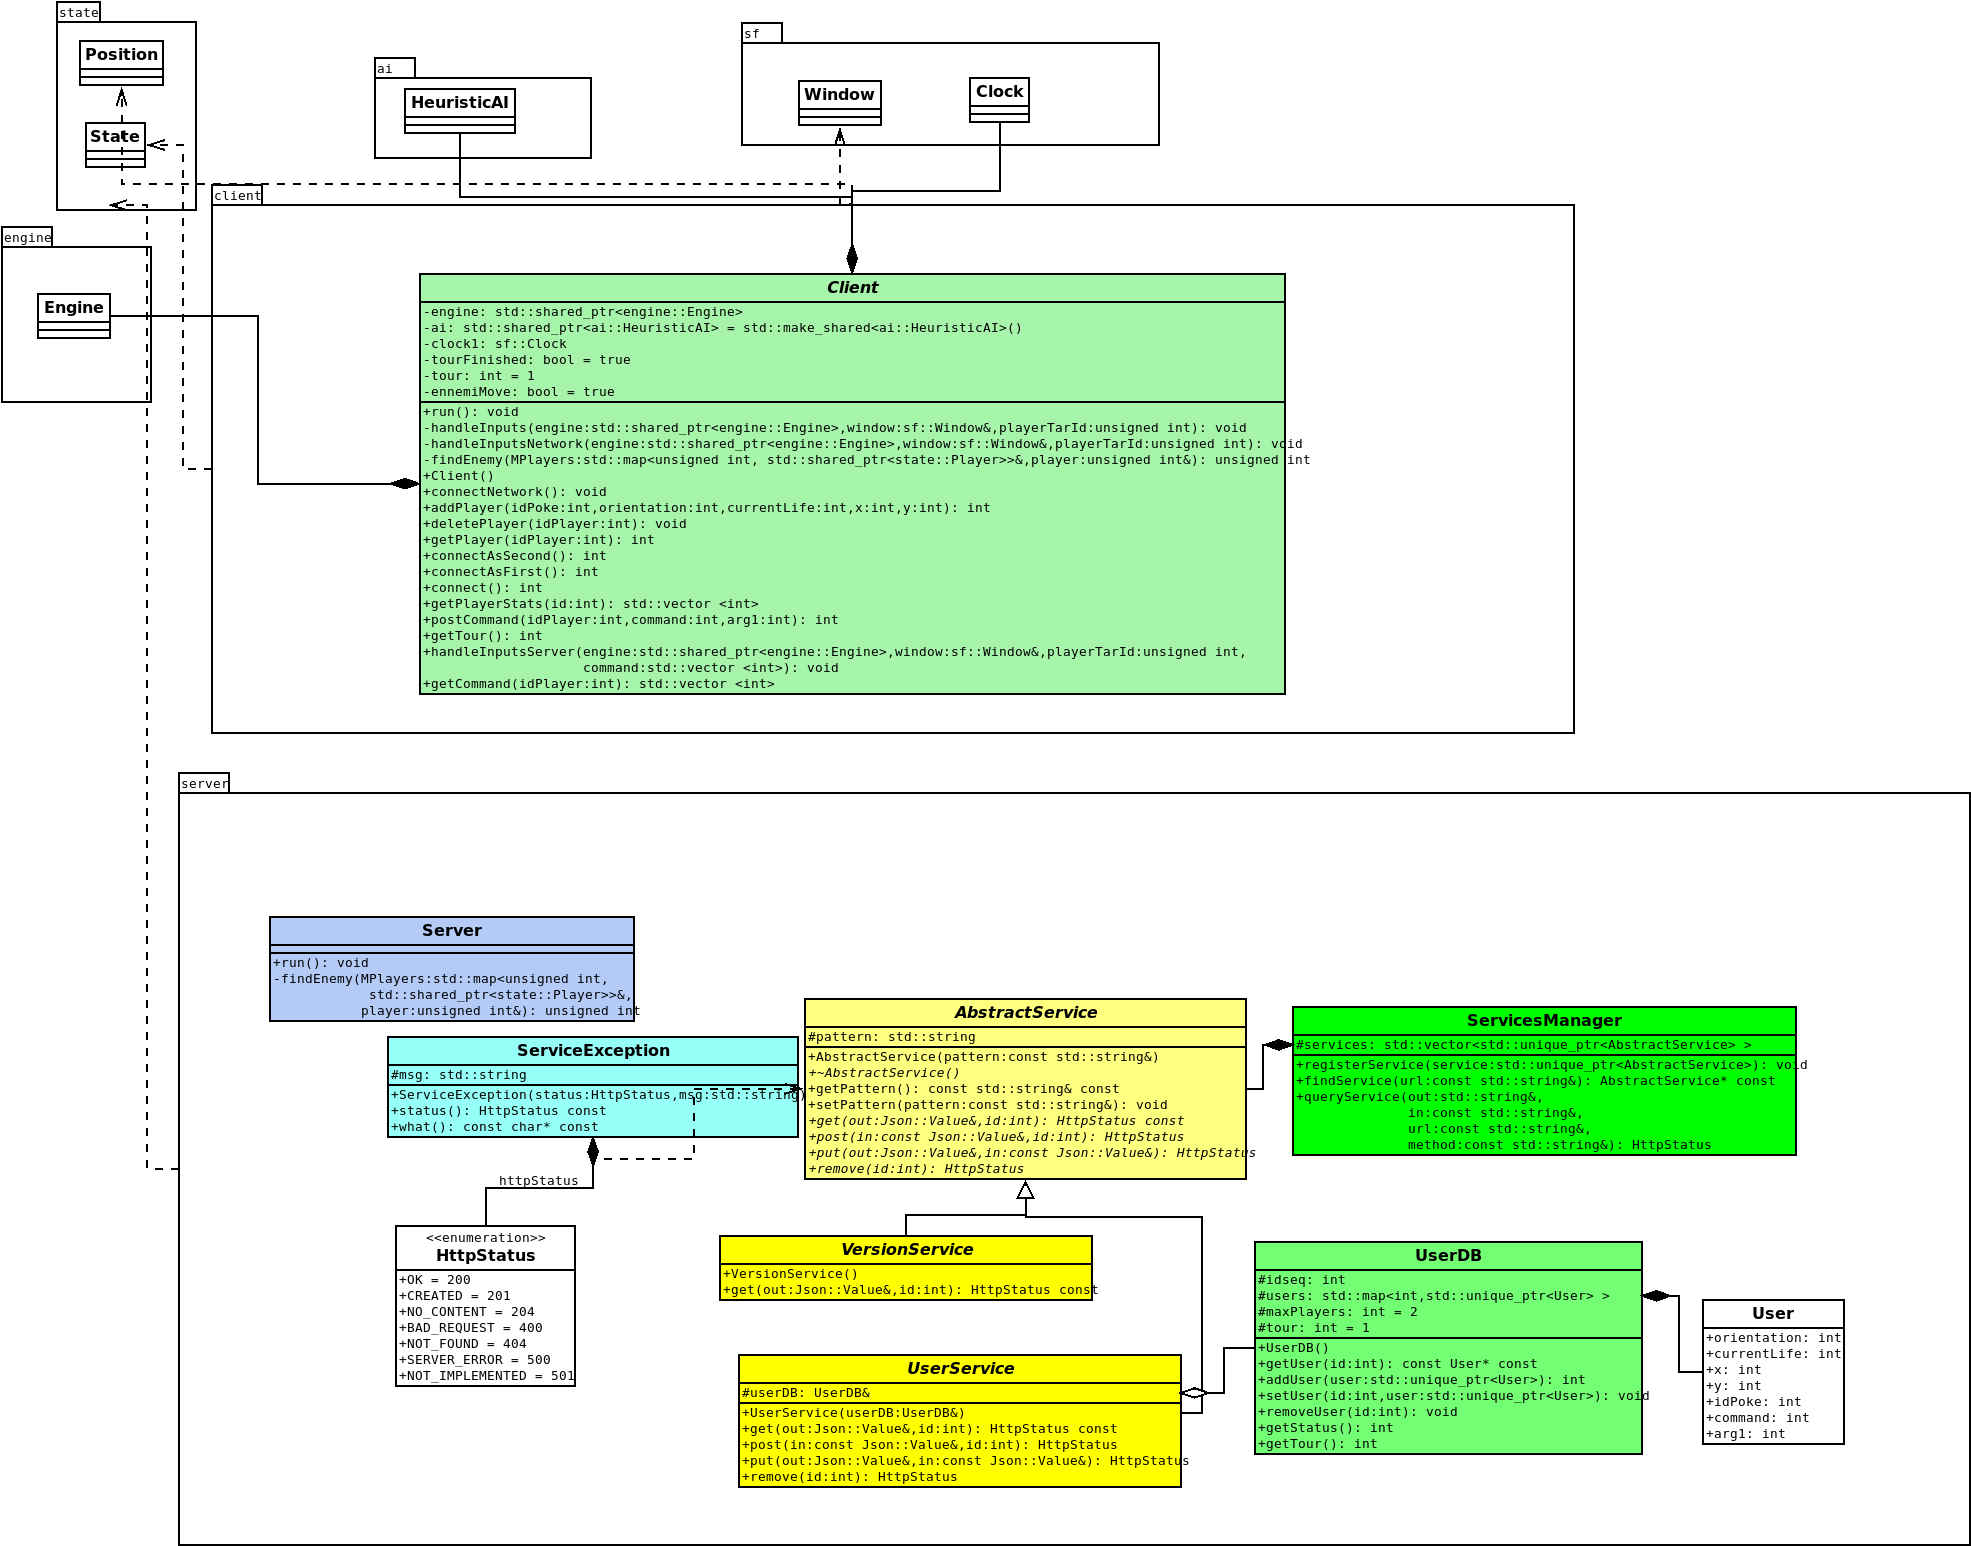
\includegraphics[width=0.9\paperheight]{module.pdf}
    %\caption{\label{uml:module}Diagramme des classes pour la modularisation.}
    %\end{figure}
    %\end{landscape}

\end{document}
